%%%%%%%%%%%%%%%%%%%%%%%%%%%%%%%%%%%
%\subsection{Fluid Dynamics Simulations}
%\label{sec:fdgen-slow-cryo-cfd}
% P. Strons
% S. Gollapinni

% restart here

Significant discrepancies between real data and simulations can have potential impacts on detector performance, as simulation results contribute to decisions about where to locate sensors and monitors, as well as definitions of various calibration quantities. However, methods of mitigating such risks include well established convergence criteria, sensitivity studies, and comparison to results of previous \dshort{cfd} simulation work by SDSU and \fnal. Additionally, the simulation will be improved with input from temperature measurements and validation tests. 

%%%%% Must find better pictures. Just use this for now %%% anne to here Fri 4/27
\begin{dunefigure}[\dshort{cfd} example]{fig:cfd-example}
  {Distribution of temperature on a plane intersecting an inlet (right) and halfway between an inlet and an outlet (left), as predicted by SDSU \dshort{cfd} simulations \cite{docdb-5915}. (See Figure\ \ref{fig:cfd-example-geometry} for geometry.)}
  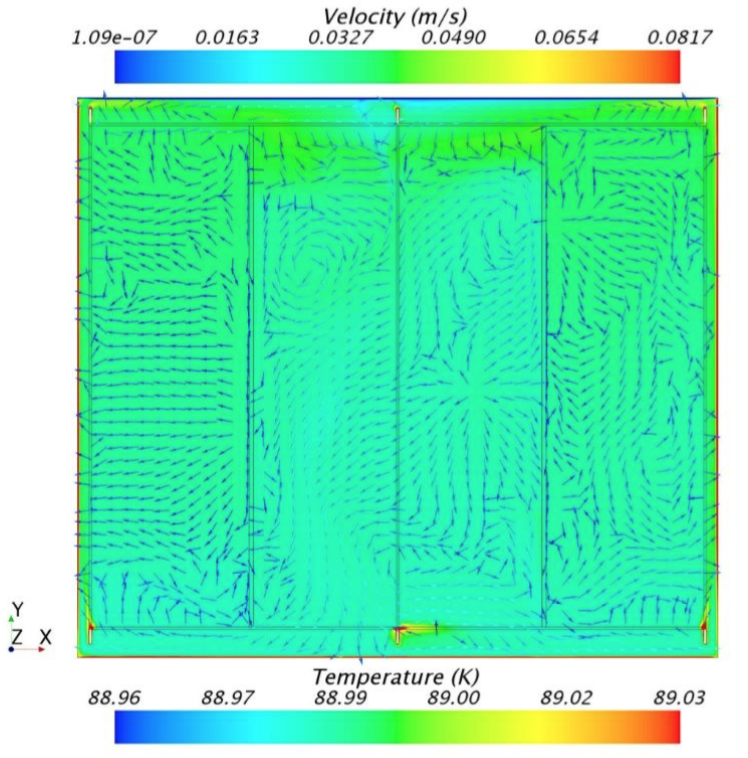
\includegraphics[height=0.4\textwidth]{cisc_cfd_outlet_z0.png}
  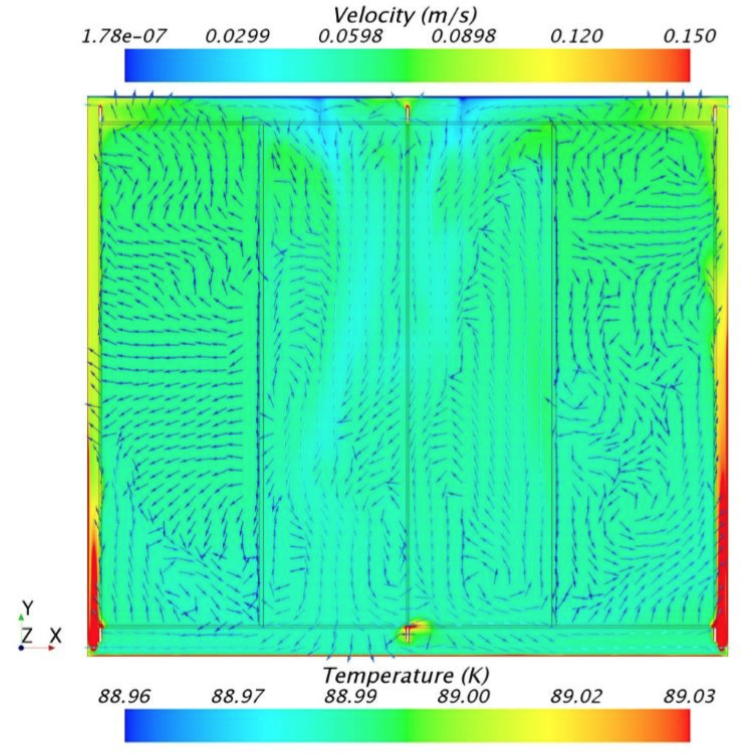
\includegraphics[height=0.4\textwidth]{cisc_cfd_inlet_z52.png}
\end{dunefigure}

Figure~\ref{fig:cfd-example} shows an example of the temperature
distribution on a plane intersecting a \dword{lar} inlet and at a
plane halfway between an inlet and an outlet; the geometry used for
this simulation is shown in Figure~\ref{fig:cfd-example-geometry}.
Note the plume of higher temperature \dword{lar} between the walls and
the outer \dword{apa} on the inlet plane.  The current locations of instrumentation in
the cryostat as shown in Figure~\ref{fig:sp-slow-cryo-ports} were
determined using the temperature and impurity distributions from these
previous simulations.

\begin{dunefigure}[\dshort{cfd} example geometry]{fig:cfd-example-geometry}
  {Layout of the \dshort{tpc} within the cryostat (top) and positions of
    \dword{lar} inlets and outlets (bottom) as modeled in the SDSU
    \dshort{cfd} simulations \cite{docdb-5915}.
    The Y axis is vertical and the X axis is parallel to the \dword{tpc}
    drift direction.
    Inlets are shown in green and outlets are shown in red.}
  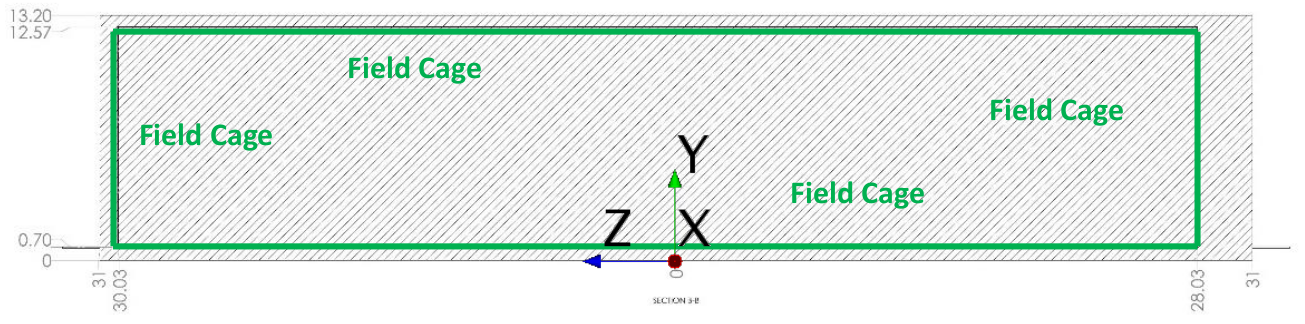
\includegraphics[width=0.8\textwidth]{cisc_cfd_cryostat-layout}
  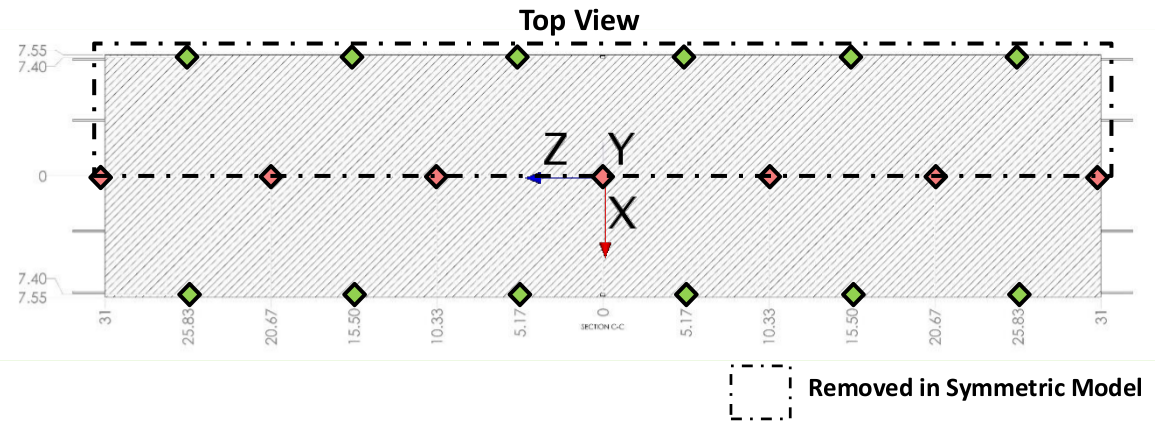
\includegraphics[width=0.8\textwidth]{cisc_cfd_inlet-outlet-layout}
\end{dunefigure}

The initial strategy for the future \dword{cfd} simulation effort is to understand the performance of \dword{protodune} cryogenics system and model the \dwords{fd} to derive requirements for instrumentation devices.
The following is a prioritized set of studies planned to help drive the requirements for other systems:
\begin{enumerate}
\item Review the DUNE \dword{fd} cryogenics system design and verify the current implementation in simulation; this is important to ensure that the model represents what will be built.
\item Model the \dword{pddp}  liquid and gas regions with the same precision as the \dword{fd}. Presently only the liquid model exists. The liquid model is needed to interpret the thermometer data, and the gas model is needed to understand how to place thermometers in the ullage and verify the design of the gaseous argon purge system.
\item Perform a \dword{cfd} study to determine the feasibility of a wier for \dual; this helps to determine if it can be used to clean the \lar surface before the extraction grid is submerged in the \dword{dpmod}.
\item Verify the \dword{spmod} \single \dword{cfd} model in simulation performed by LBNF; this defines the requirements for instrumentation devices (e.g., thermometry).
\item Model the \dword{pddp} liquid and gas regions with the same precision as the \dword{fd}. \fixme{same as a previous bullet}
\end{enumerate}
